\documentclass{beamer}
\setbeamertemplate{navigation symbols}{}
\setbeamertemplate{footline}[frame number]{}
\usepackage[italian]{babel}
\usepackage{multicol}
\usepackage{newlfont}
\usepackage{color}
\usepackage{hyperref}
\usepackage{xcolor}
\usepackage{graphicx}
\usepackage{caption}
\usepackage{subcaption}
\usepackage{multirow}

\definecolor{unibo}{RGB}{182,53,47}
\definecolor{hclue_blue}{RGB}{123,150,191}
\definecolor{hclue_yellow}{RGB}{214,187,113}
\definecolor{hclue_green}{RGB}{138,177,112}
\definecolor{hclue_red}{RGB}{213,166,163}

\mode<presentation>
\usecolortheme{seahorse}
\usefonttheme{default}   
\setbeamercolor*{palette primary}{bg=unibo}
\setbeamercolor*{palette secondary}{bg=unibo, fg = white}
\setbeamercolor*{palette tertiary}{bg=unibo, fg = white}
\setbeamercolor*{titlelike}{fg=unibo}
\setbeamercolor*{title}{bg=unibo}
\setbeamercolor*{item}{fg=unibo}
\setbeamercolor*{caption name}{fg=unibo}

\hypersetup{
    colorlinks=true,
    linkcolor=black,
    filecolor=magenta,
    urlcolor=blue,
}



\title{Development of a heterogeneous clustering algorithm for particle shower reconstruction in high energy physics using the SYCL abstraction layer}

\author{Luca Ferragina \\ \vspace{15mm} {\small Relatore: Francesco Giacomini \\ \hspace{-5mm} \vspace{2mm}{\small Correlatore: Felice Pantaleo}}}



\date{21 Ottobre 2022}

\begin{document}

{\setbeamertemplate{footline}{} 
\begin{frame}[noframenumbering]
\maketitle
\end{frame}
}

\begin{frame}{Gli aggiornamenti di LHC e degli esperimenti}
Nella ricerca di nuova fisica, il Large Hadron Collider al CERN viene aggiornato periodicamente in due modi:
\begin{itemize}
    \item \textbf{Aumentando l'energia} dei fasci di protoni che collidono
    \item \textbf{Incrementando} il numero di collisioni al secondo (\textbf{luminosità})
\end{itemize}

Gli esperimenti si aggiornano a loro volta per sfruttare le nuove potenzialità dell'acceleratore.

\hspace{10mm}

Nel 2029 è previsto un miglioramento sostanziale della luminosità integrata per collisioni protone-protone (incremento $\sim$ \textbf{10x}): \textbf{High Luminosity LHC (HL-LHC)}.

\end{frame}

\begin{frame}{Il nuovo calorimetro di CMS pone sfide computazionali notevoli}
L'endcap calorimeter HGCAL avrà sezioni elettromagnetica e adronica ad alta granularità ($\sim$ 6 milioni di canali).

\begin{figure}
    \centering
    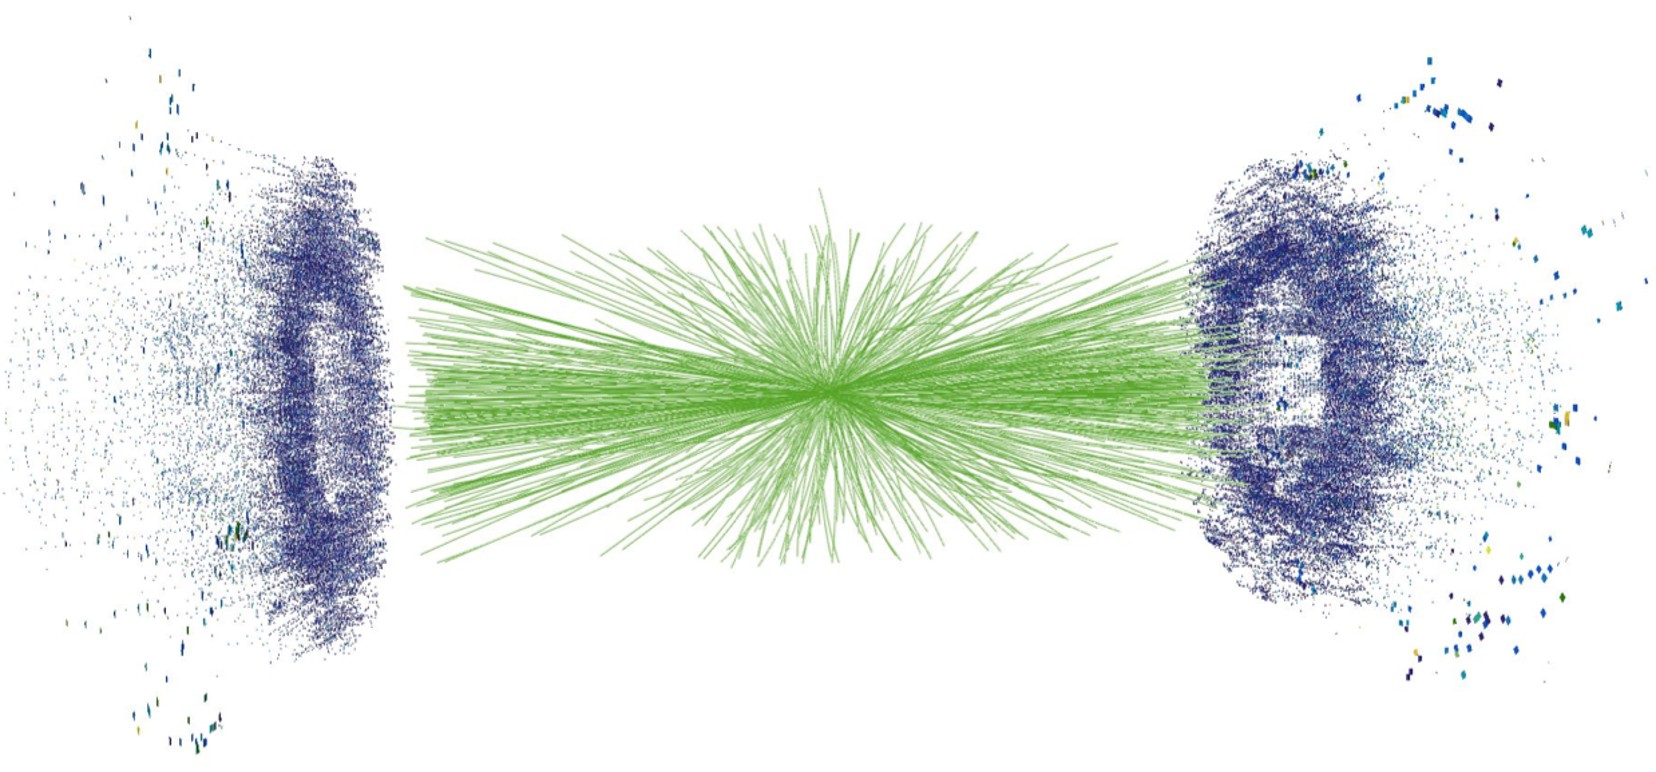
\includegraphics[width=0.8\textwidth]{media/presentazione/particle_shower.png}
\end{figure}

\textbf{Crescita} dei \textbf{dati acquisiti} e \textbf{tempo limitato} per selezionare gli eventi. Ricerca di soluzioni per \textbf{aumentare il throughput}\footnote{Eventi ricostruiti per unità di tempo.}.

\end{frame}

\begin{frame}{Il calcolo eterogeneo come soluzione}
Il gruppo Patatrack di CMS ha già cominciato a esplorare le potenzialità del \textbf{calcolo eterogeneo} per la ricostruzione.
\vspace{3mm}
\begin{columns}
\column{0.4\linewidth}
\centering
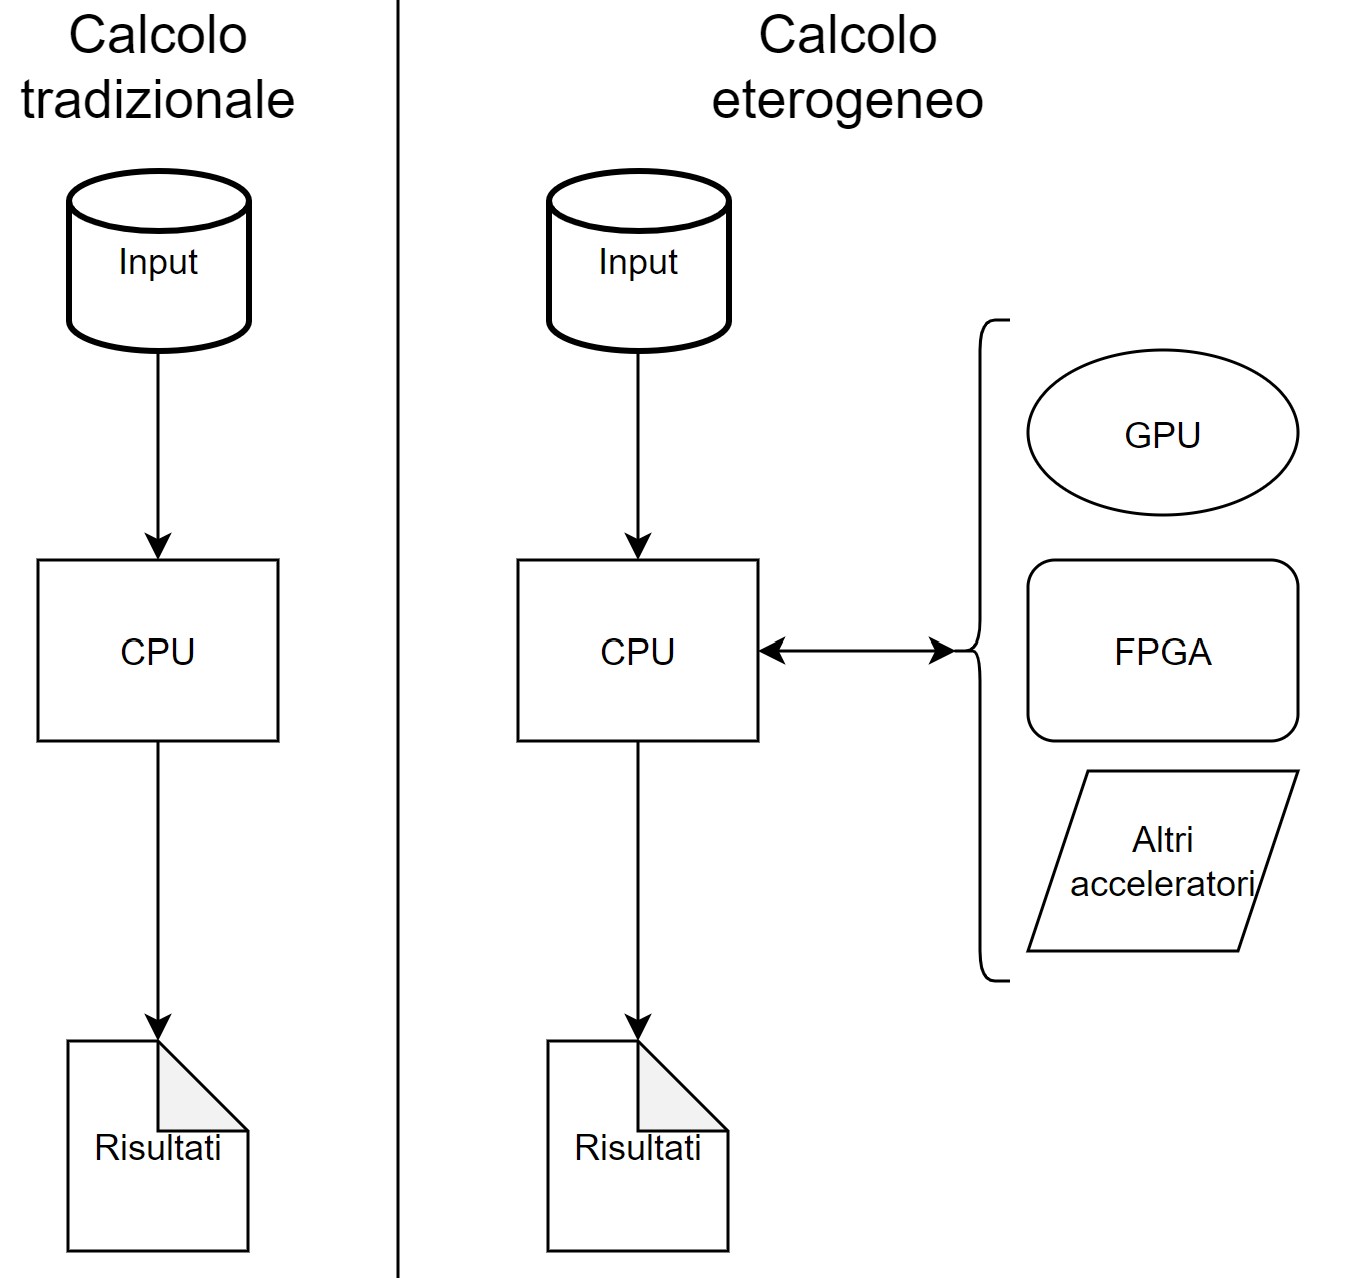
\includegraphics[width=\textwidth]{media/calcolo_eterogeneo.png}
\column{0.6\linewidth}
\begin{itemize}
    \item Parte della computazione può essere eseguita su dispositivi diversi dalla CPU (host)
    \item Le GPU offrono possibilità di eseguire codice parallelo in maniera estremamente efficiente
    \item Dimostrato \textbf{incremento delle prestazioni fino a 3 volte} con risultati compatibili
    \end{itemize}
\end{columns}
\vspace{3mm}
\textbf{Difficoltà} nel mantenere e tradurre il codice per \textbf{diverse architetture e dispositivi}.
\end{frame}

\begin{frame}{Portabilità di codice e prestazioni con compatibility layer}
I compatibility layer permettono di:
\begin{itemize}
    \item Scrivere un \textbf{unico} codice sorgente per produrre un file eseguibile su più architetture
    \item \textbf{Limitare} al minimo la \textbf{perdita di prestazioni} rispetto al codice nativo di ciascuna architettura
    \item \textbf{Semplificazione} nella \textbf{manutenzione} e \textbf{sviluppo} di codice
\end{itemize}

Due layer in analisi per prossime Run di LHC:
\vspace{3mm}
\begin{columns}

\vspace{3mm}

\column{0.3\linewidth}

\includegraphics[width=\textwidth]{media/alpaka.png}

\vspace{3mm}


\includegraphics[width=\textwidth]{media/sycl.png}
\column{0.7\linewidth}
\begin{itemize}
    \item Alpaka: production nella prossima fase di Run3: singolo codice per CPU e NVIDIA GPUs
    \item SYCL: in fase di sperimentazione, sviluppo attivo con l'implementazione di Intel: \textbf{oneAPI}
\end{itemize}
\end{columns}

\end{frame}

\begin{frame}{Il caso specifico di CLUE: clustering eterogeneo}
Sviluppare algoritmi per \textbf{architetture eterogenee} richiede di \textbf{ripensare al problema} dall'inizio cercando di sfruttare al meglio le possibilità di \textbf{parallelizzazione}.
\begin{figure}
    \centering
    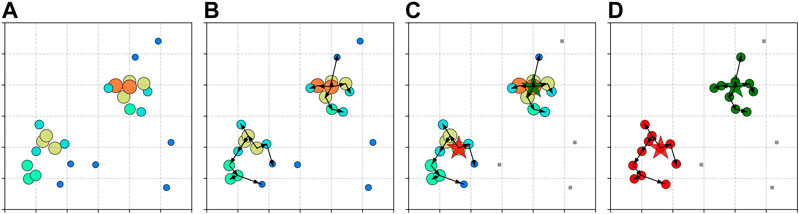
\includegraphics[width=0.8\textwidth]{media/clustering_procedure.jpg}
\end{figure}

\begin{columns}
\column{0.7\linewidth}
\textbf{\href{https://www.frontiersin.org/articles/10.3389/fdata.2020.591315/full}{CLUE}} (CLUstering of Energy): algoritmo di clustering basato sulla densità e \textbf{parallelizzabile}
\begin{enumerate}[A.]
    \item Calcolo della densità locale
    \item Assegnazione del \emph{nearest higher}
    \item Assegnazione degli status \emph{seed}, \emph{outlier} e \emph{follower}
    \item Formazione dei clusters
\end{enumerate}

\column{0.4\linewidth}
\flushleft
\begin{itemize}
    \item Calcolo di informazioni su più punti \textbf{contemporaneamente} in parallelo
    \item Le prestazioni scalano \textbf{linearmente} con il numero di punti
\end{itemize}
\end{columns}
    
\end{frame}

\begin{frame}{Introduzione al framework di CMS: il workflow di heterogeneous CLUE}
Framework \textbf{modulare} in cui ogni modulo agisce in maniera diversa sui dati. Tutti i dati si trovano all'interno di un \emph{Evento}.
\vspace{3mm}
\begin{columns}
\column{0.4\linewidth}
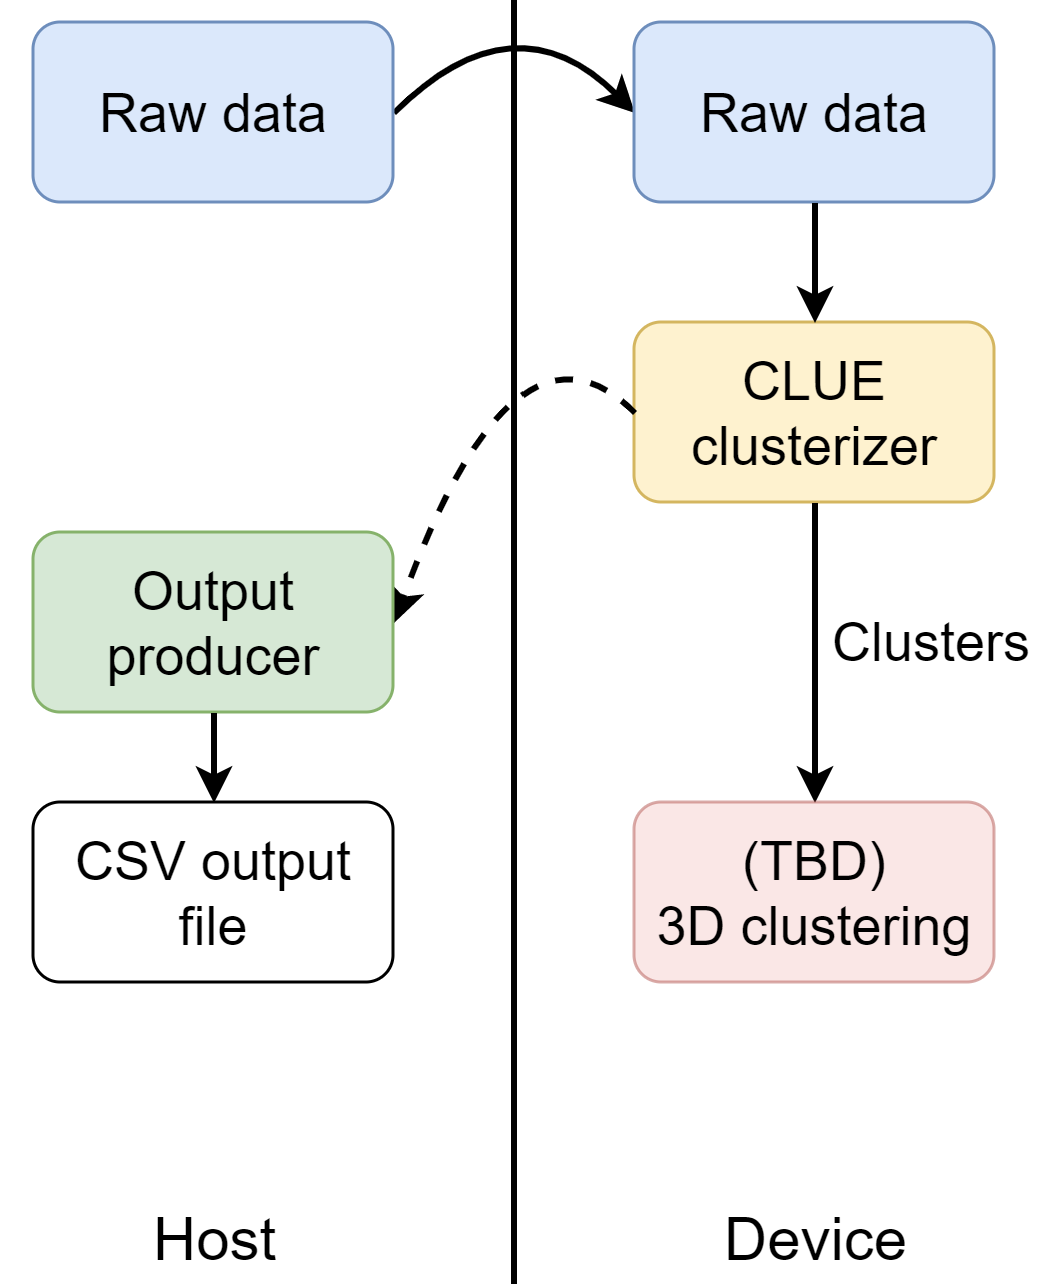
\includegraphics[width=\textwidth]{media/hclue_workflow.png}
\column{0.6\linewidth}
\begin{itemize}
    \item \textcolor{hclue_blue}{Source}: legge i dati da un file di input e li inserisce nell'\emph{Evento}
    \item \textcolor{hclue_yellow}{Producer}: legge i dati dall'\emph{Evento} e produce i clusters
    \item \textcolor{hclue_green}{Analyzer (opzionale)}: scrive i dati di ogni punto in ciascun cluster in un file unico file csv
    \item \textcolor{hclue_red}{Producer}: in sviluppo un modulo per il clustering tridimensionale
\end{itemize}
\end{columns}
\end{frame}

\begin{frame}{I risultati di heterogeneous CLUE su un intero layer}
\begin{figure}
    \centering
    \begin{subfigure}[t]{0.49\linewidth}
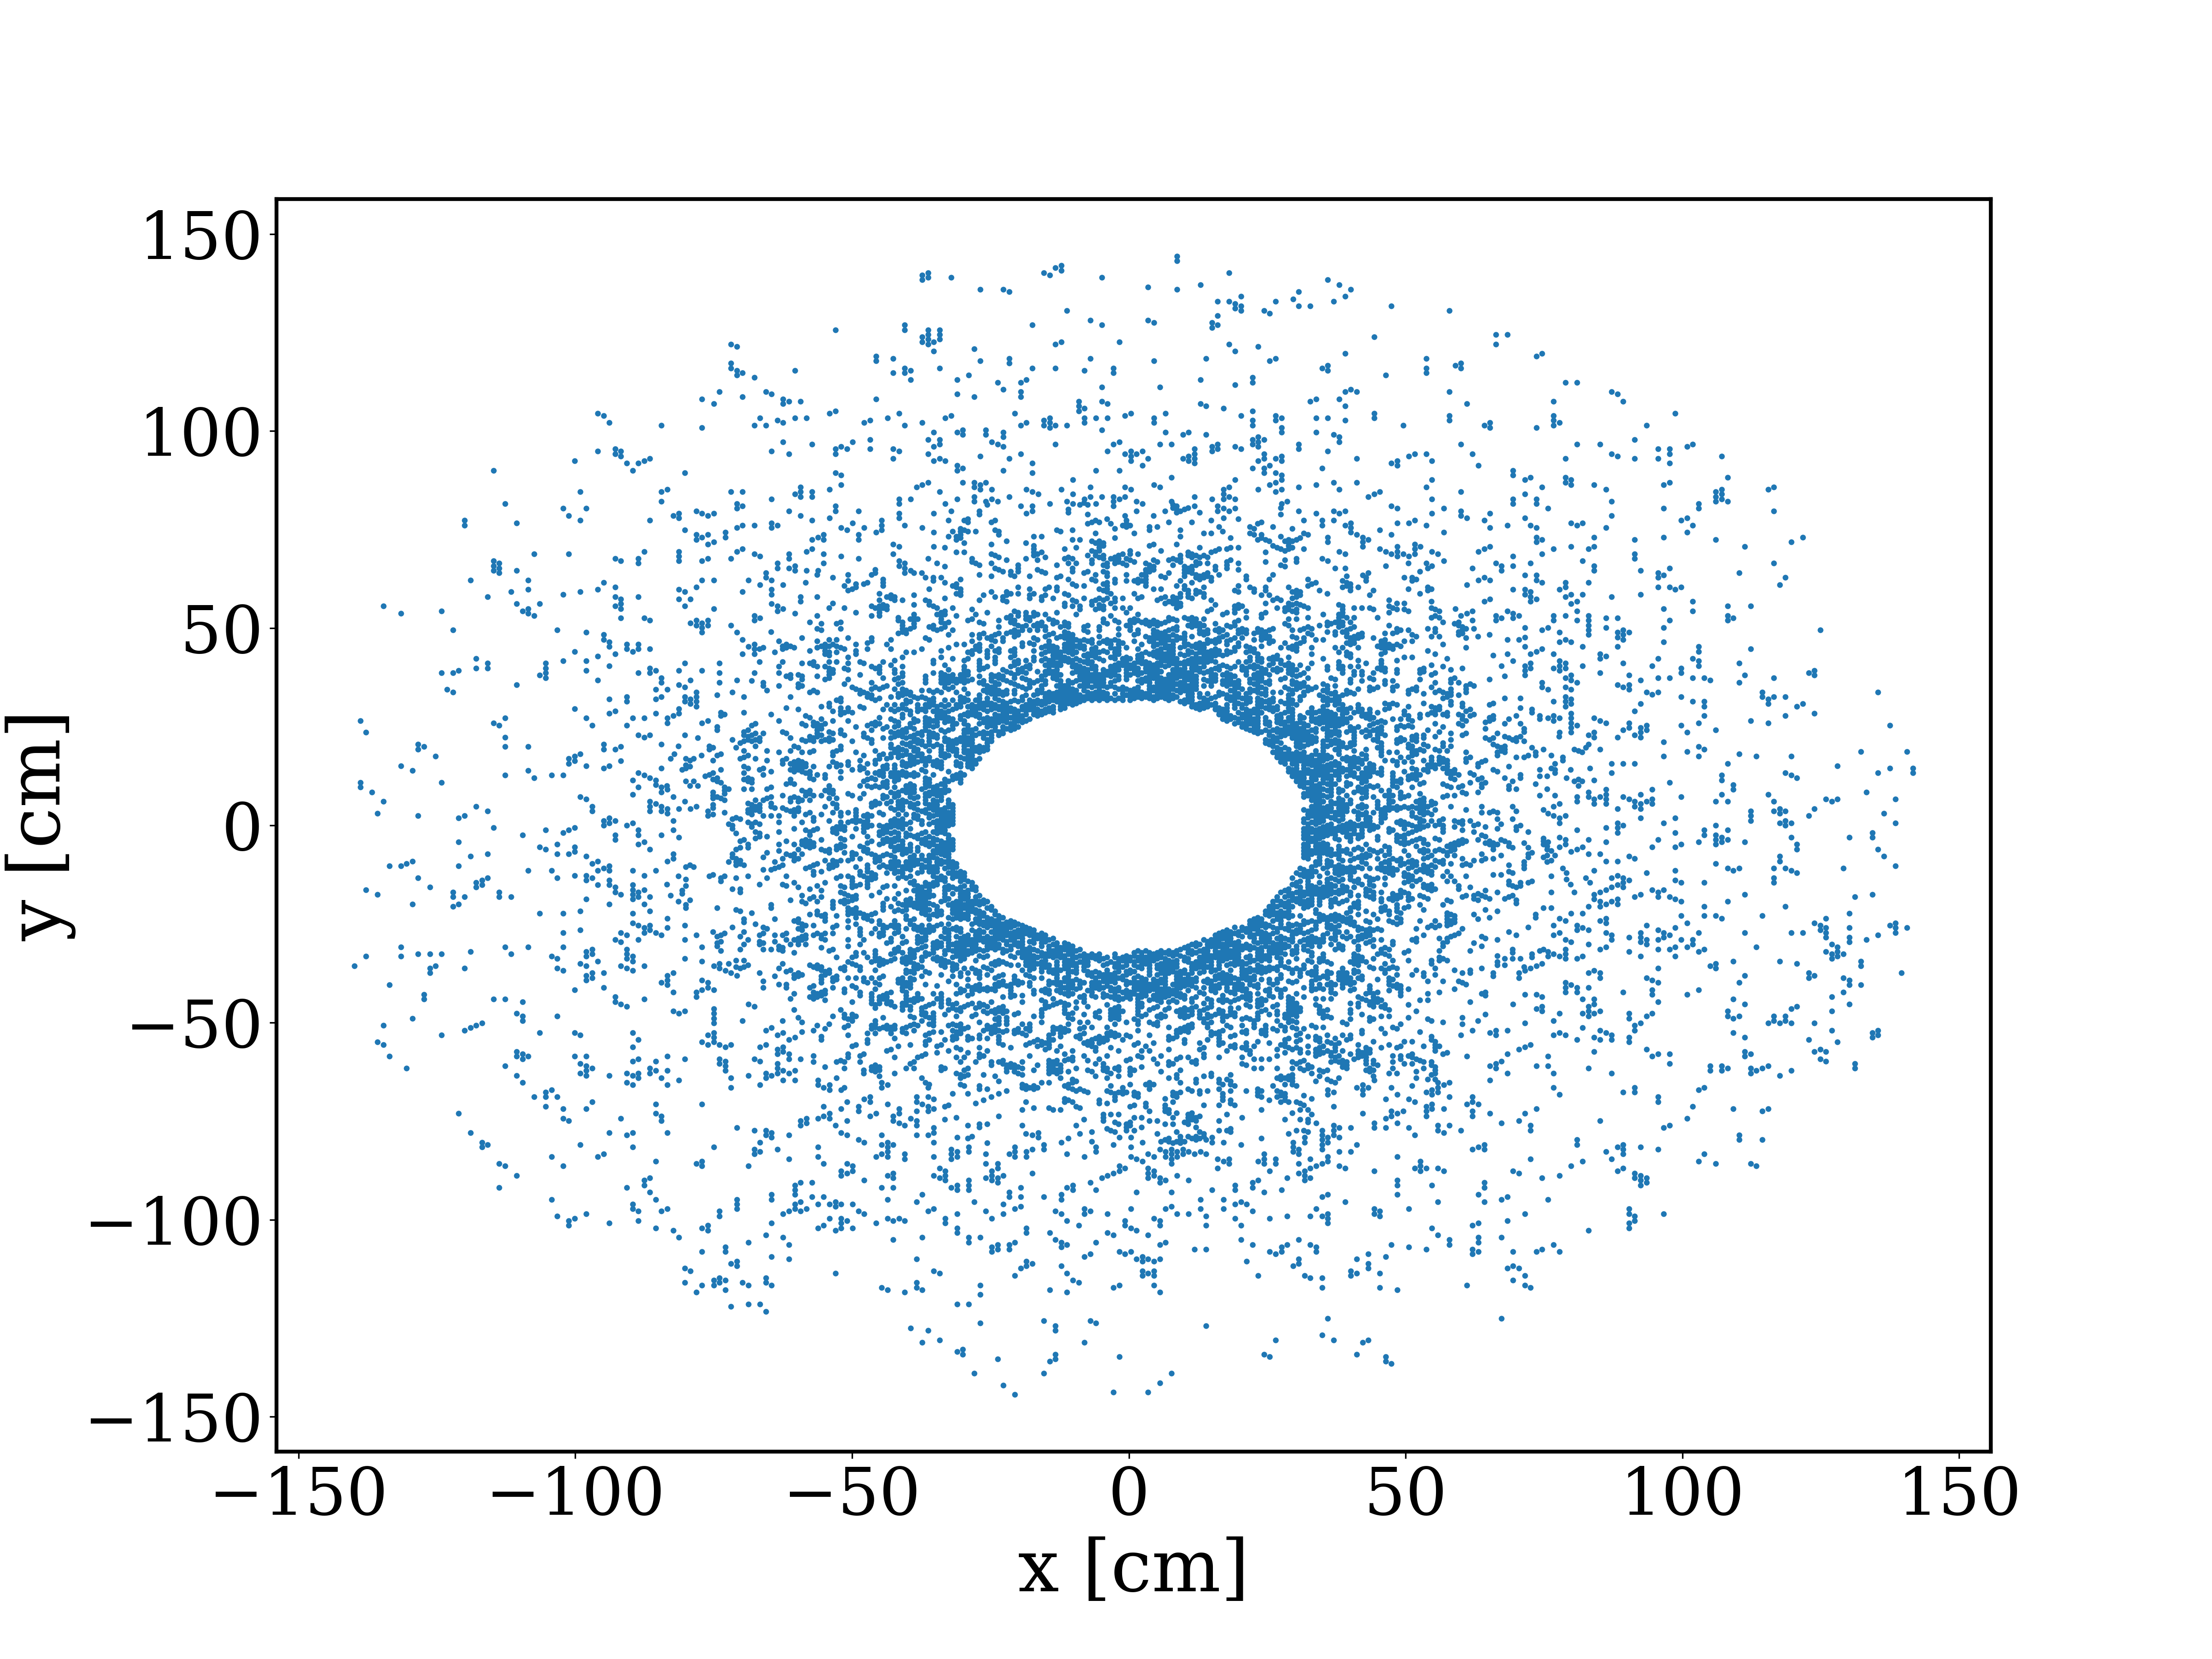
\includegraphics[width=\linewidth]{media/presentazione/whole_detector.png}
    \caption{Dati in input per il layer 5 del detector.}
    \end{subfigure}
    \hfill
    \begin{subfigure}[t]{0.49\linewidth}
        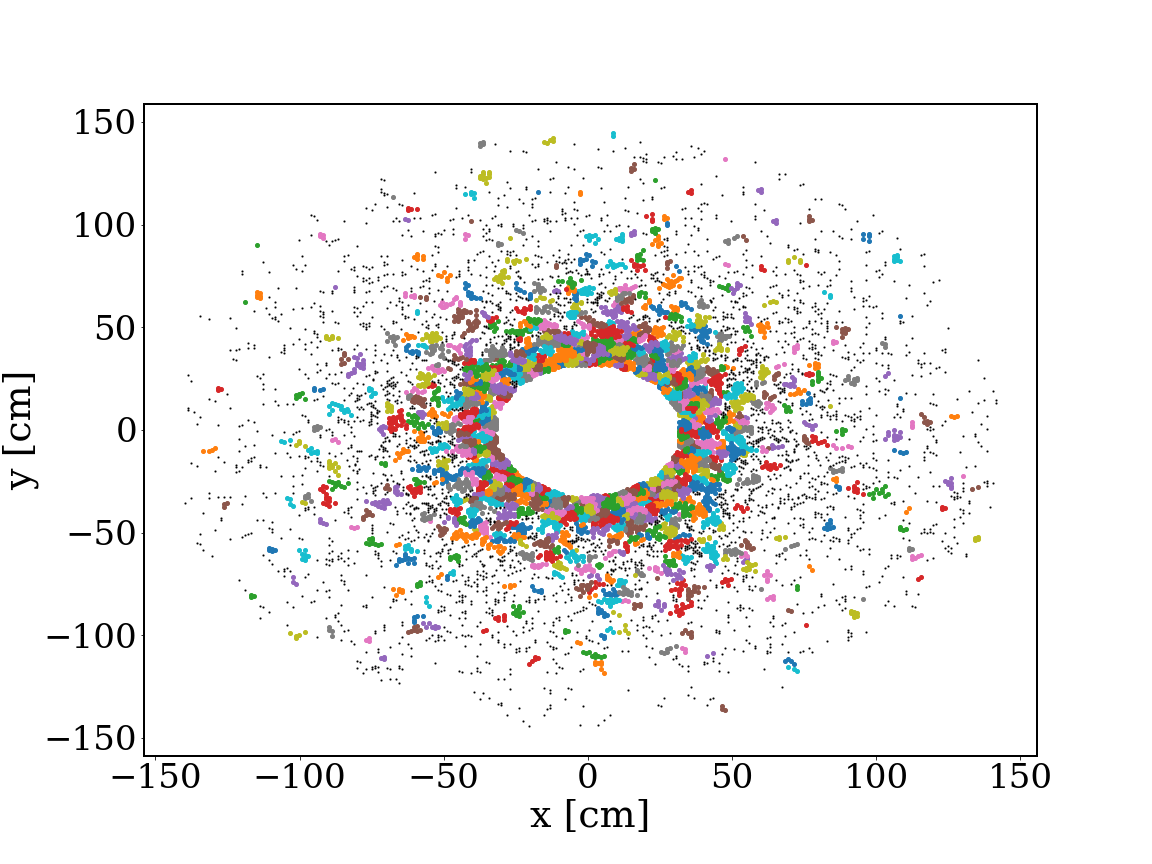
\includegraphics[width=\linewidth]{media/presentazione/clusters_whole_detector.png}
        \caption{Clusters prodotti da CLUE nel layer 5.}
    \end{subfigure}
\end{figure}

\end{frame}

\begin{frame}{Dettaglio su clusters prodotti in una finestra del detector}

\begin{figure}
    \centering
    \begin{subfigure}[c]{0.49\linewidth}
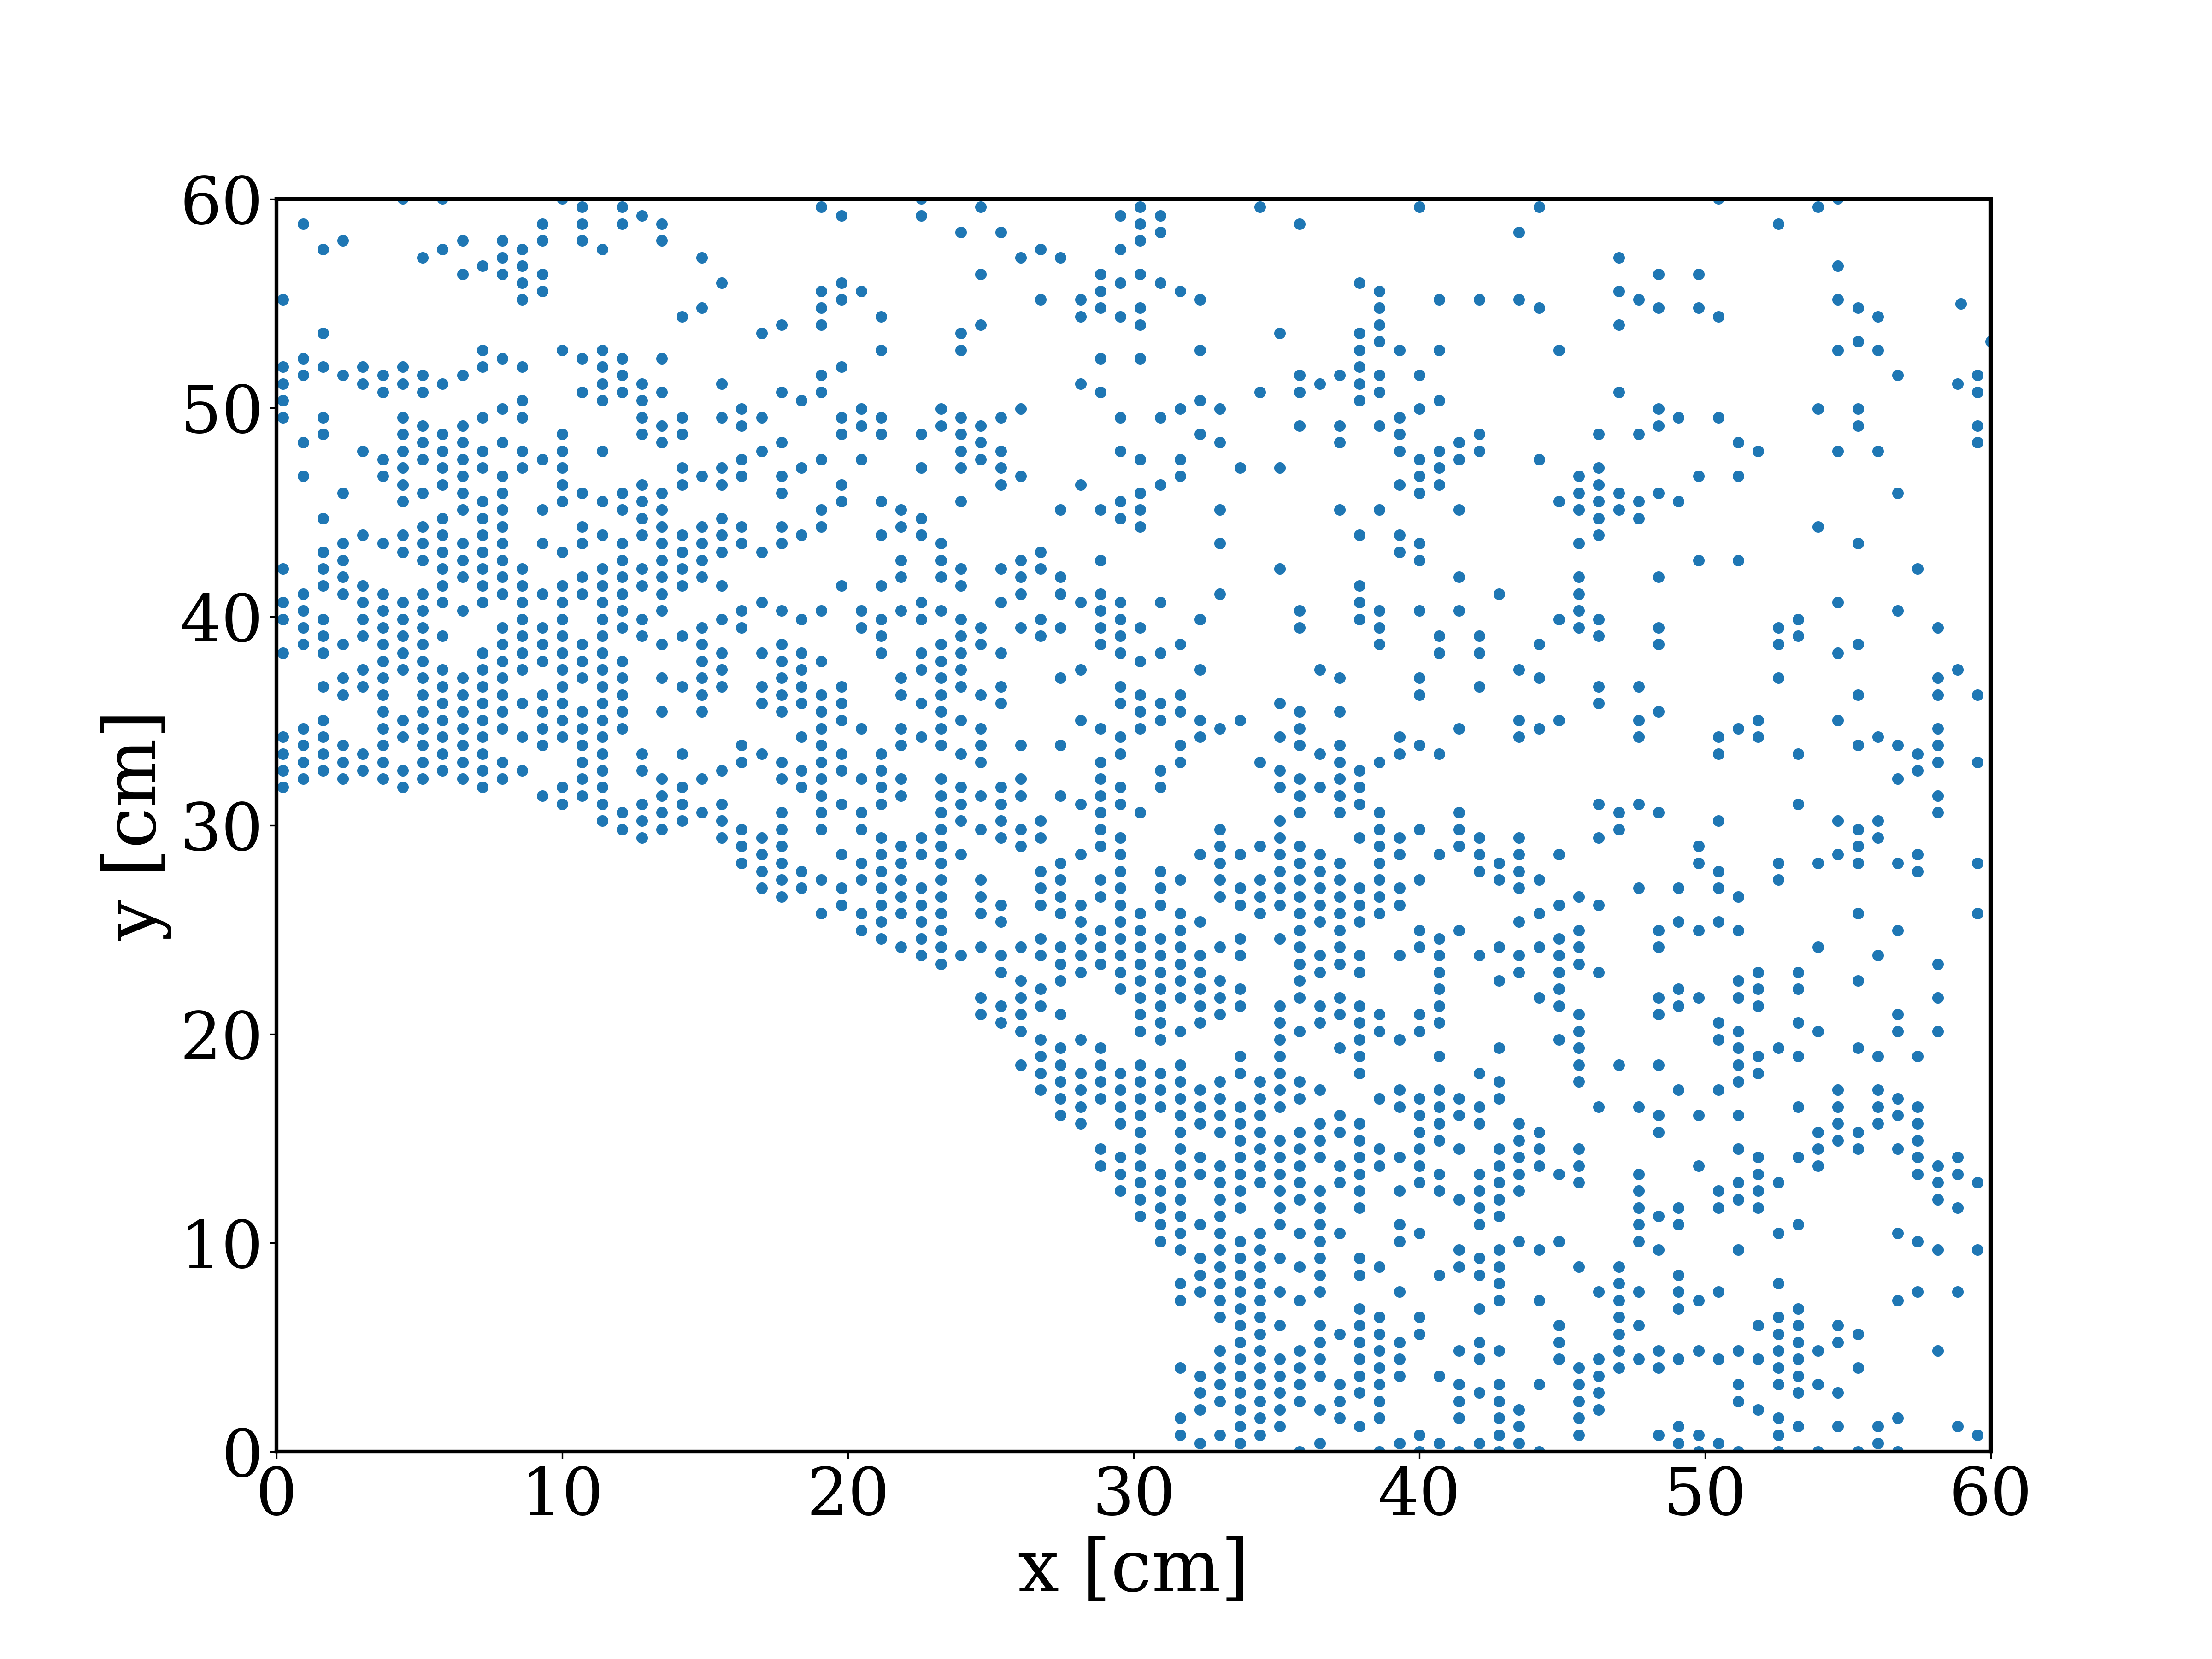
\includegraphics[width=\linewidth]{media/presentazione/detector_window.png}
    \caption{Dati in input per una piccola finestra del layer 5.}
    \end{subfigure}
    \hfill
    \begin{subfigure}[c]{0.49\linewidth}
        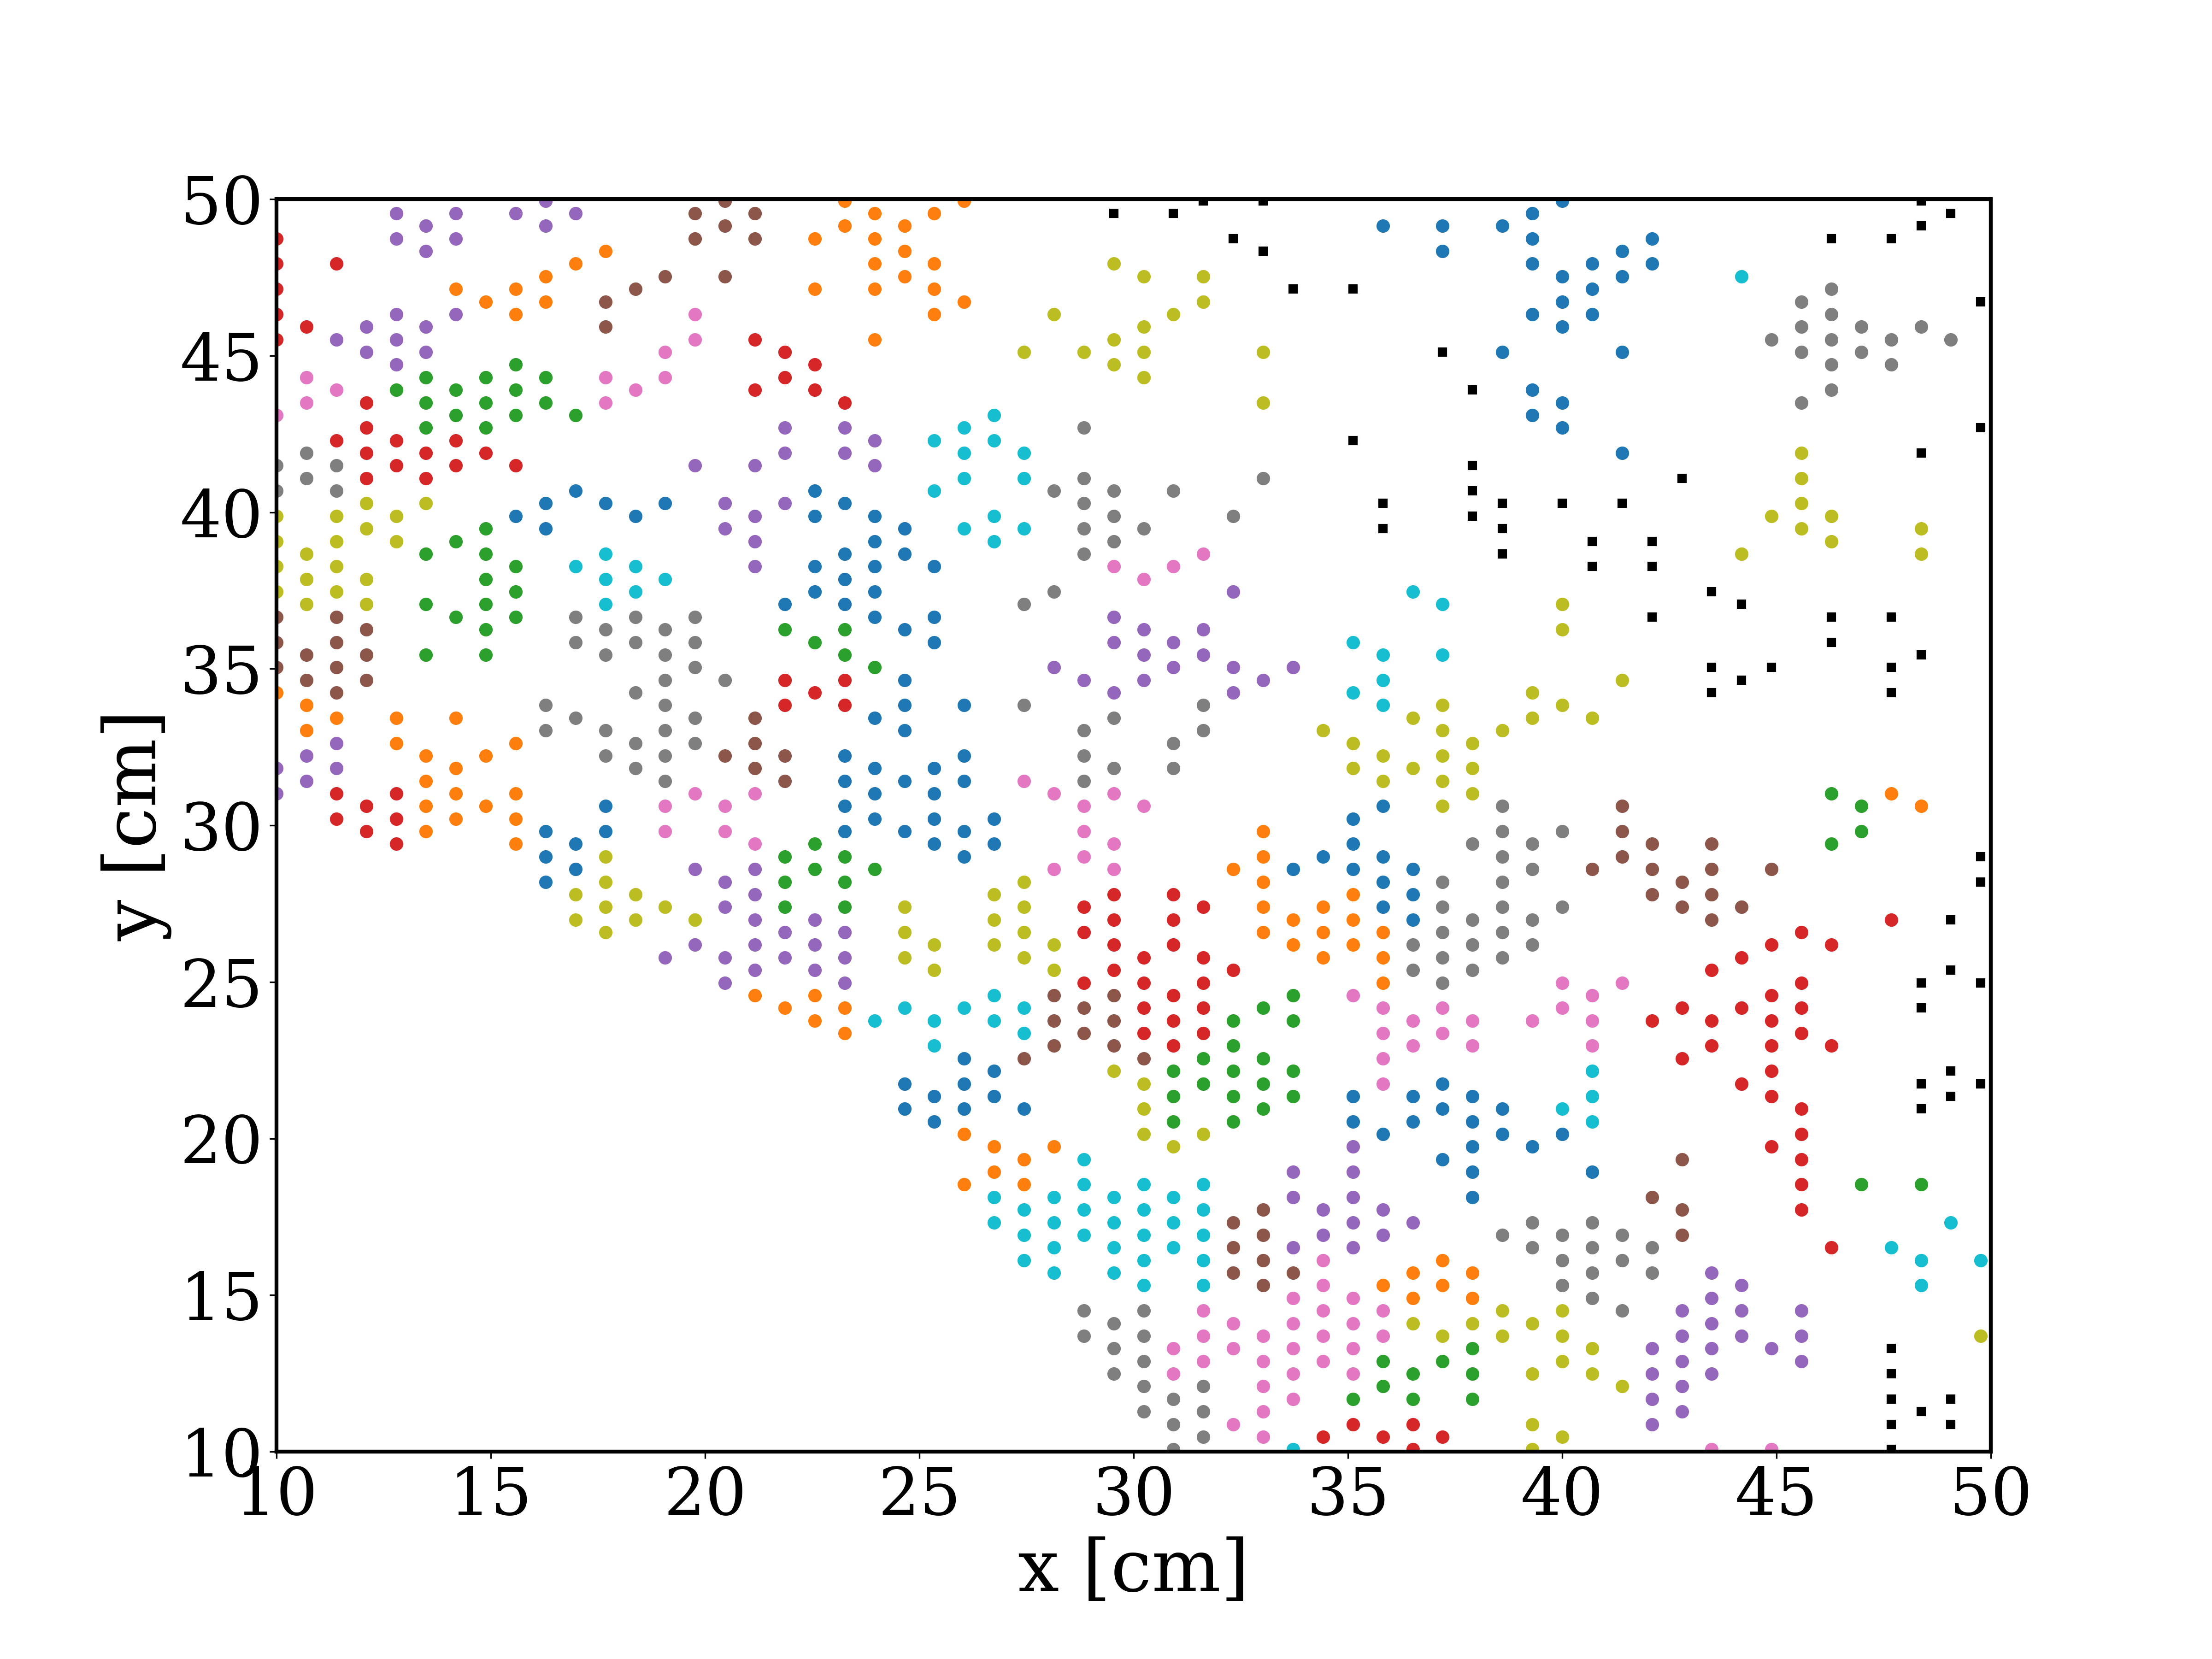
\includegraphics[width=\linewidth]{media/presentazione/clusters_detector_window.png}
        \caption{Clusters prodotti da CLUE in una piccola finestra del layer 5.}
    \end{subfigure}
\end{figure}

\end{frame}

\begin{frame}{Le performance computazionali pongono SYCL come soluzione promettente per il futuro}

\begin{figure}
    \centering
    \begin{subfigure}[t]{0.49\textwidth}
    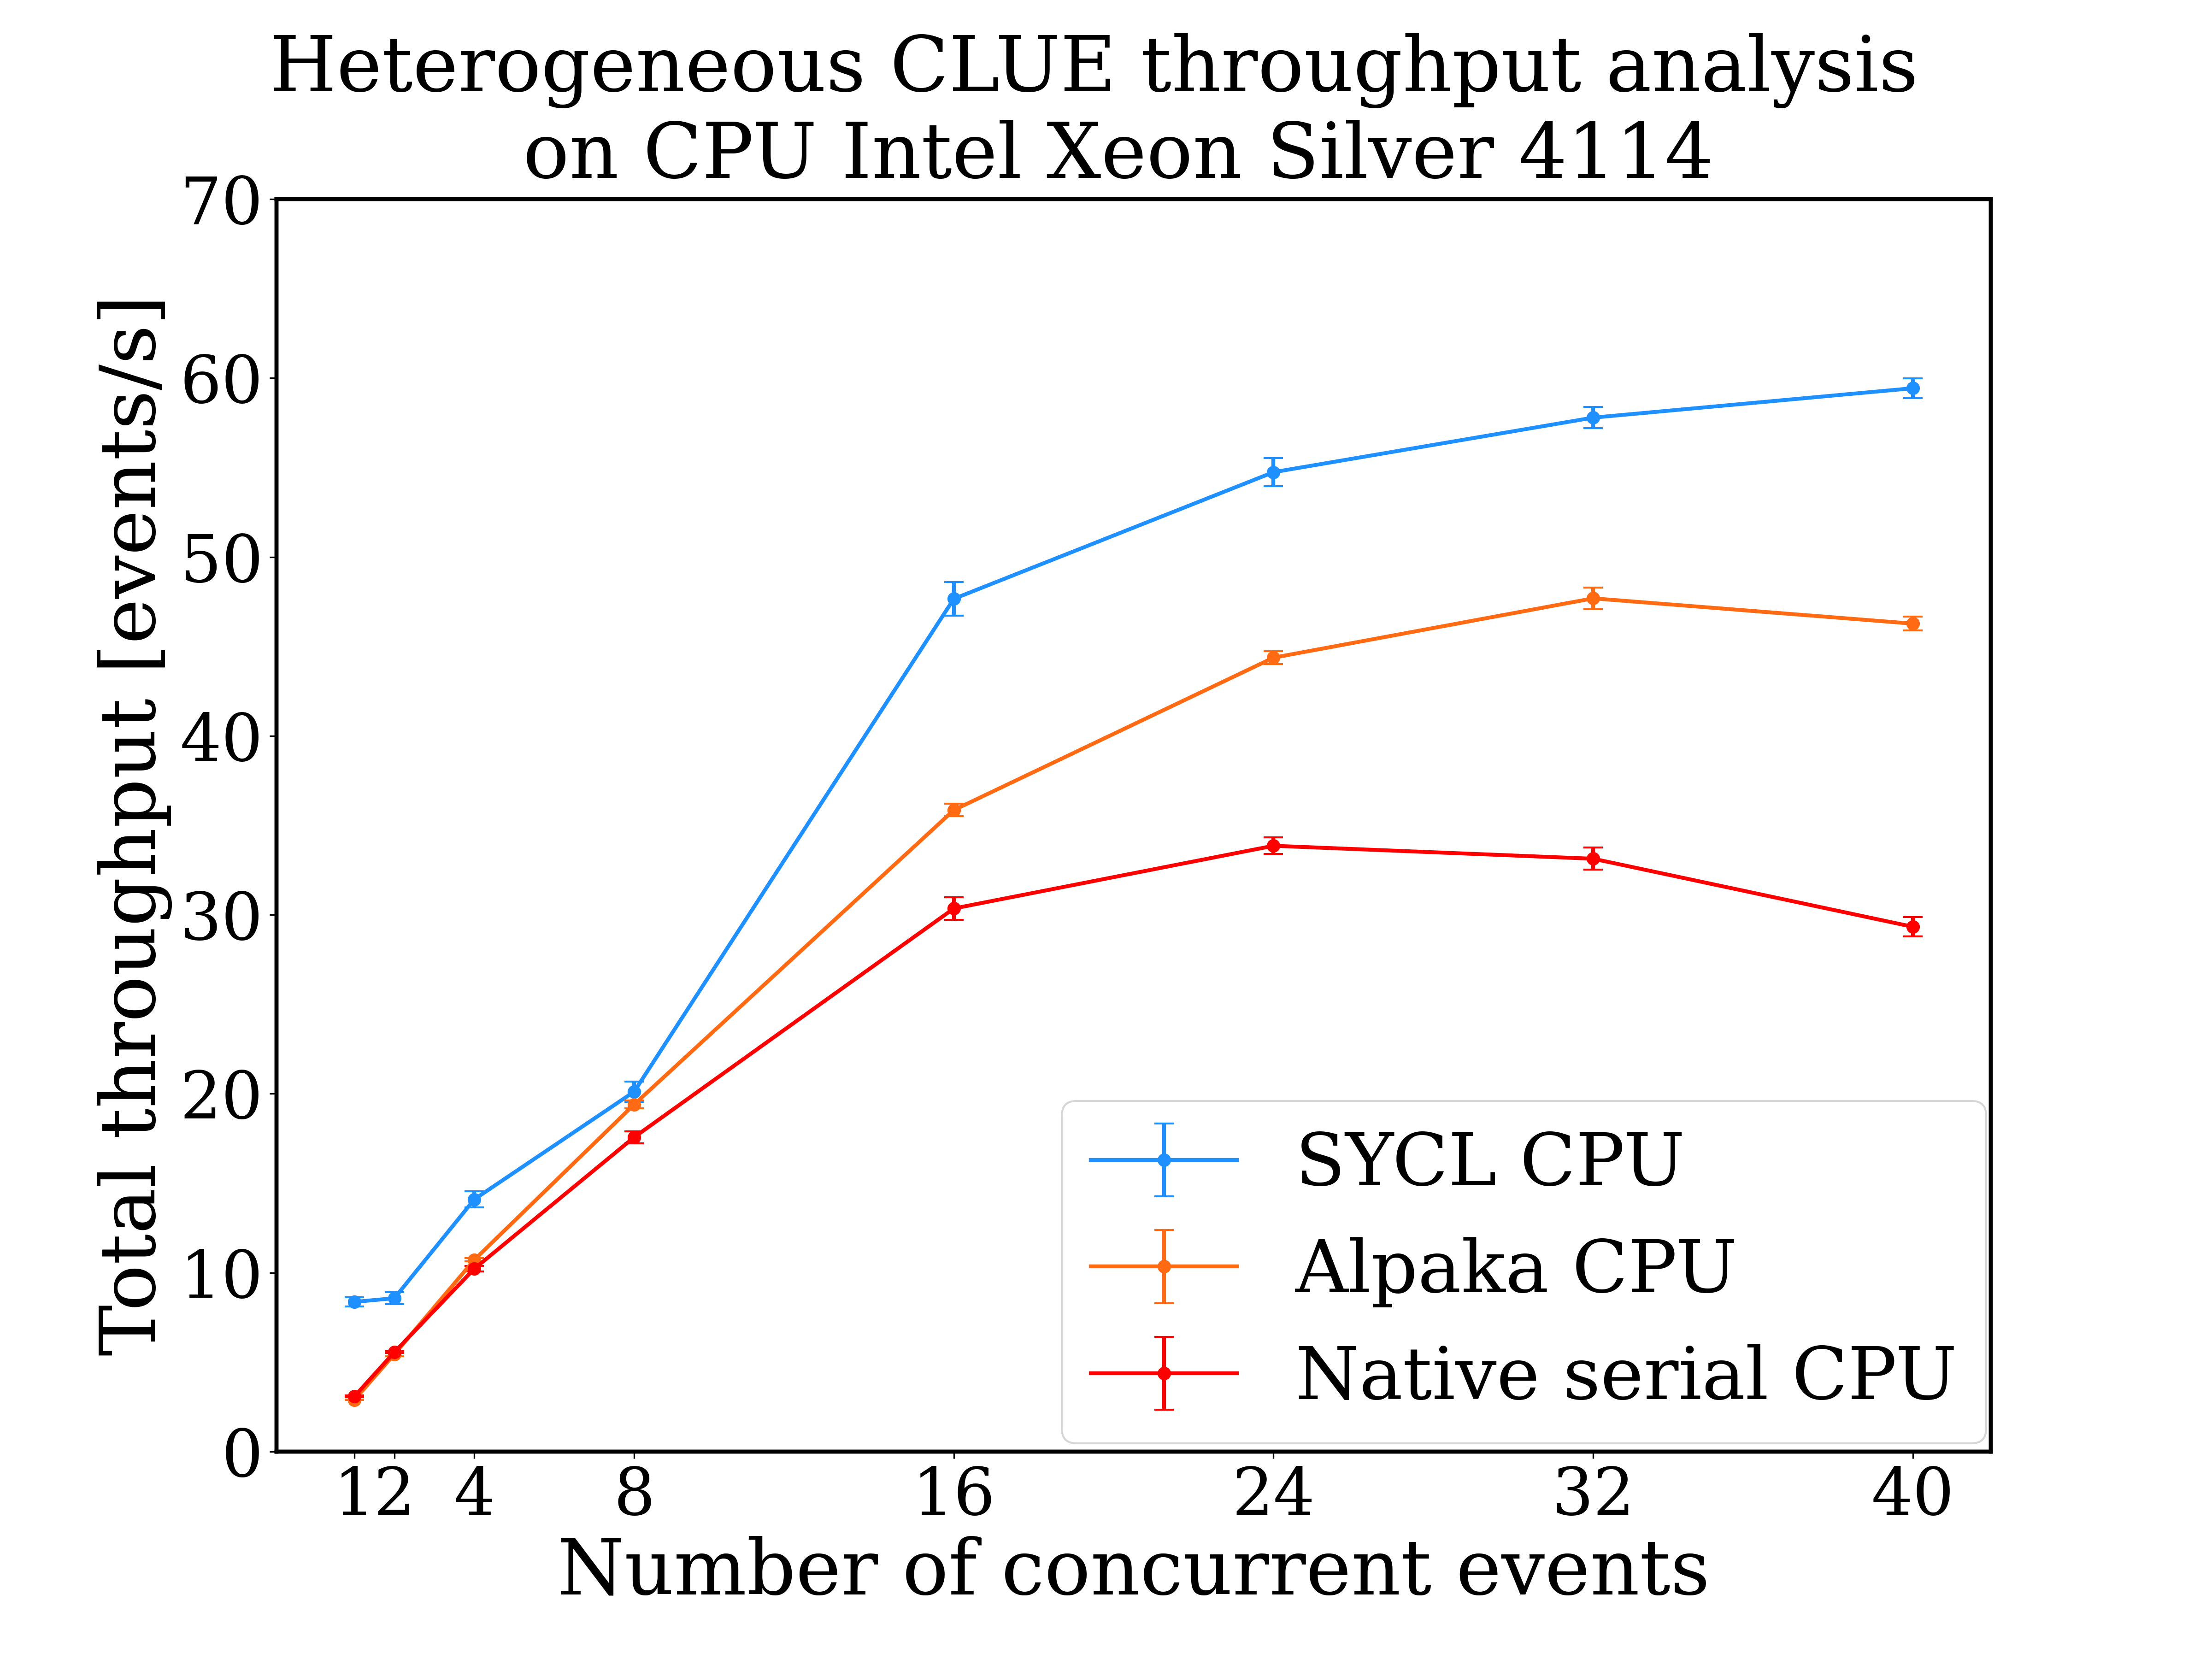
\includegraphics[width=\textwidth]{media/presentazione/hCLUE_cpu_performance.png}
    \caption{L'implementazione su CPU è più efficiente di Alpaka e del codice seriale nativo.}
    \end{subfigure}
    \begin{subfigure}[t]{0.49\textwidth}
    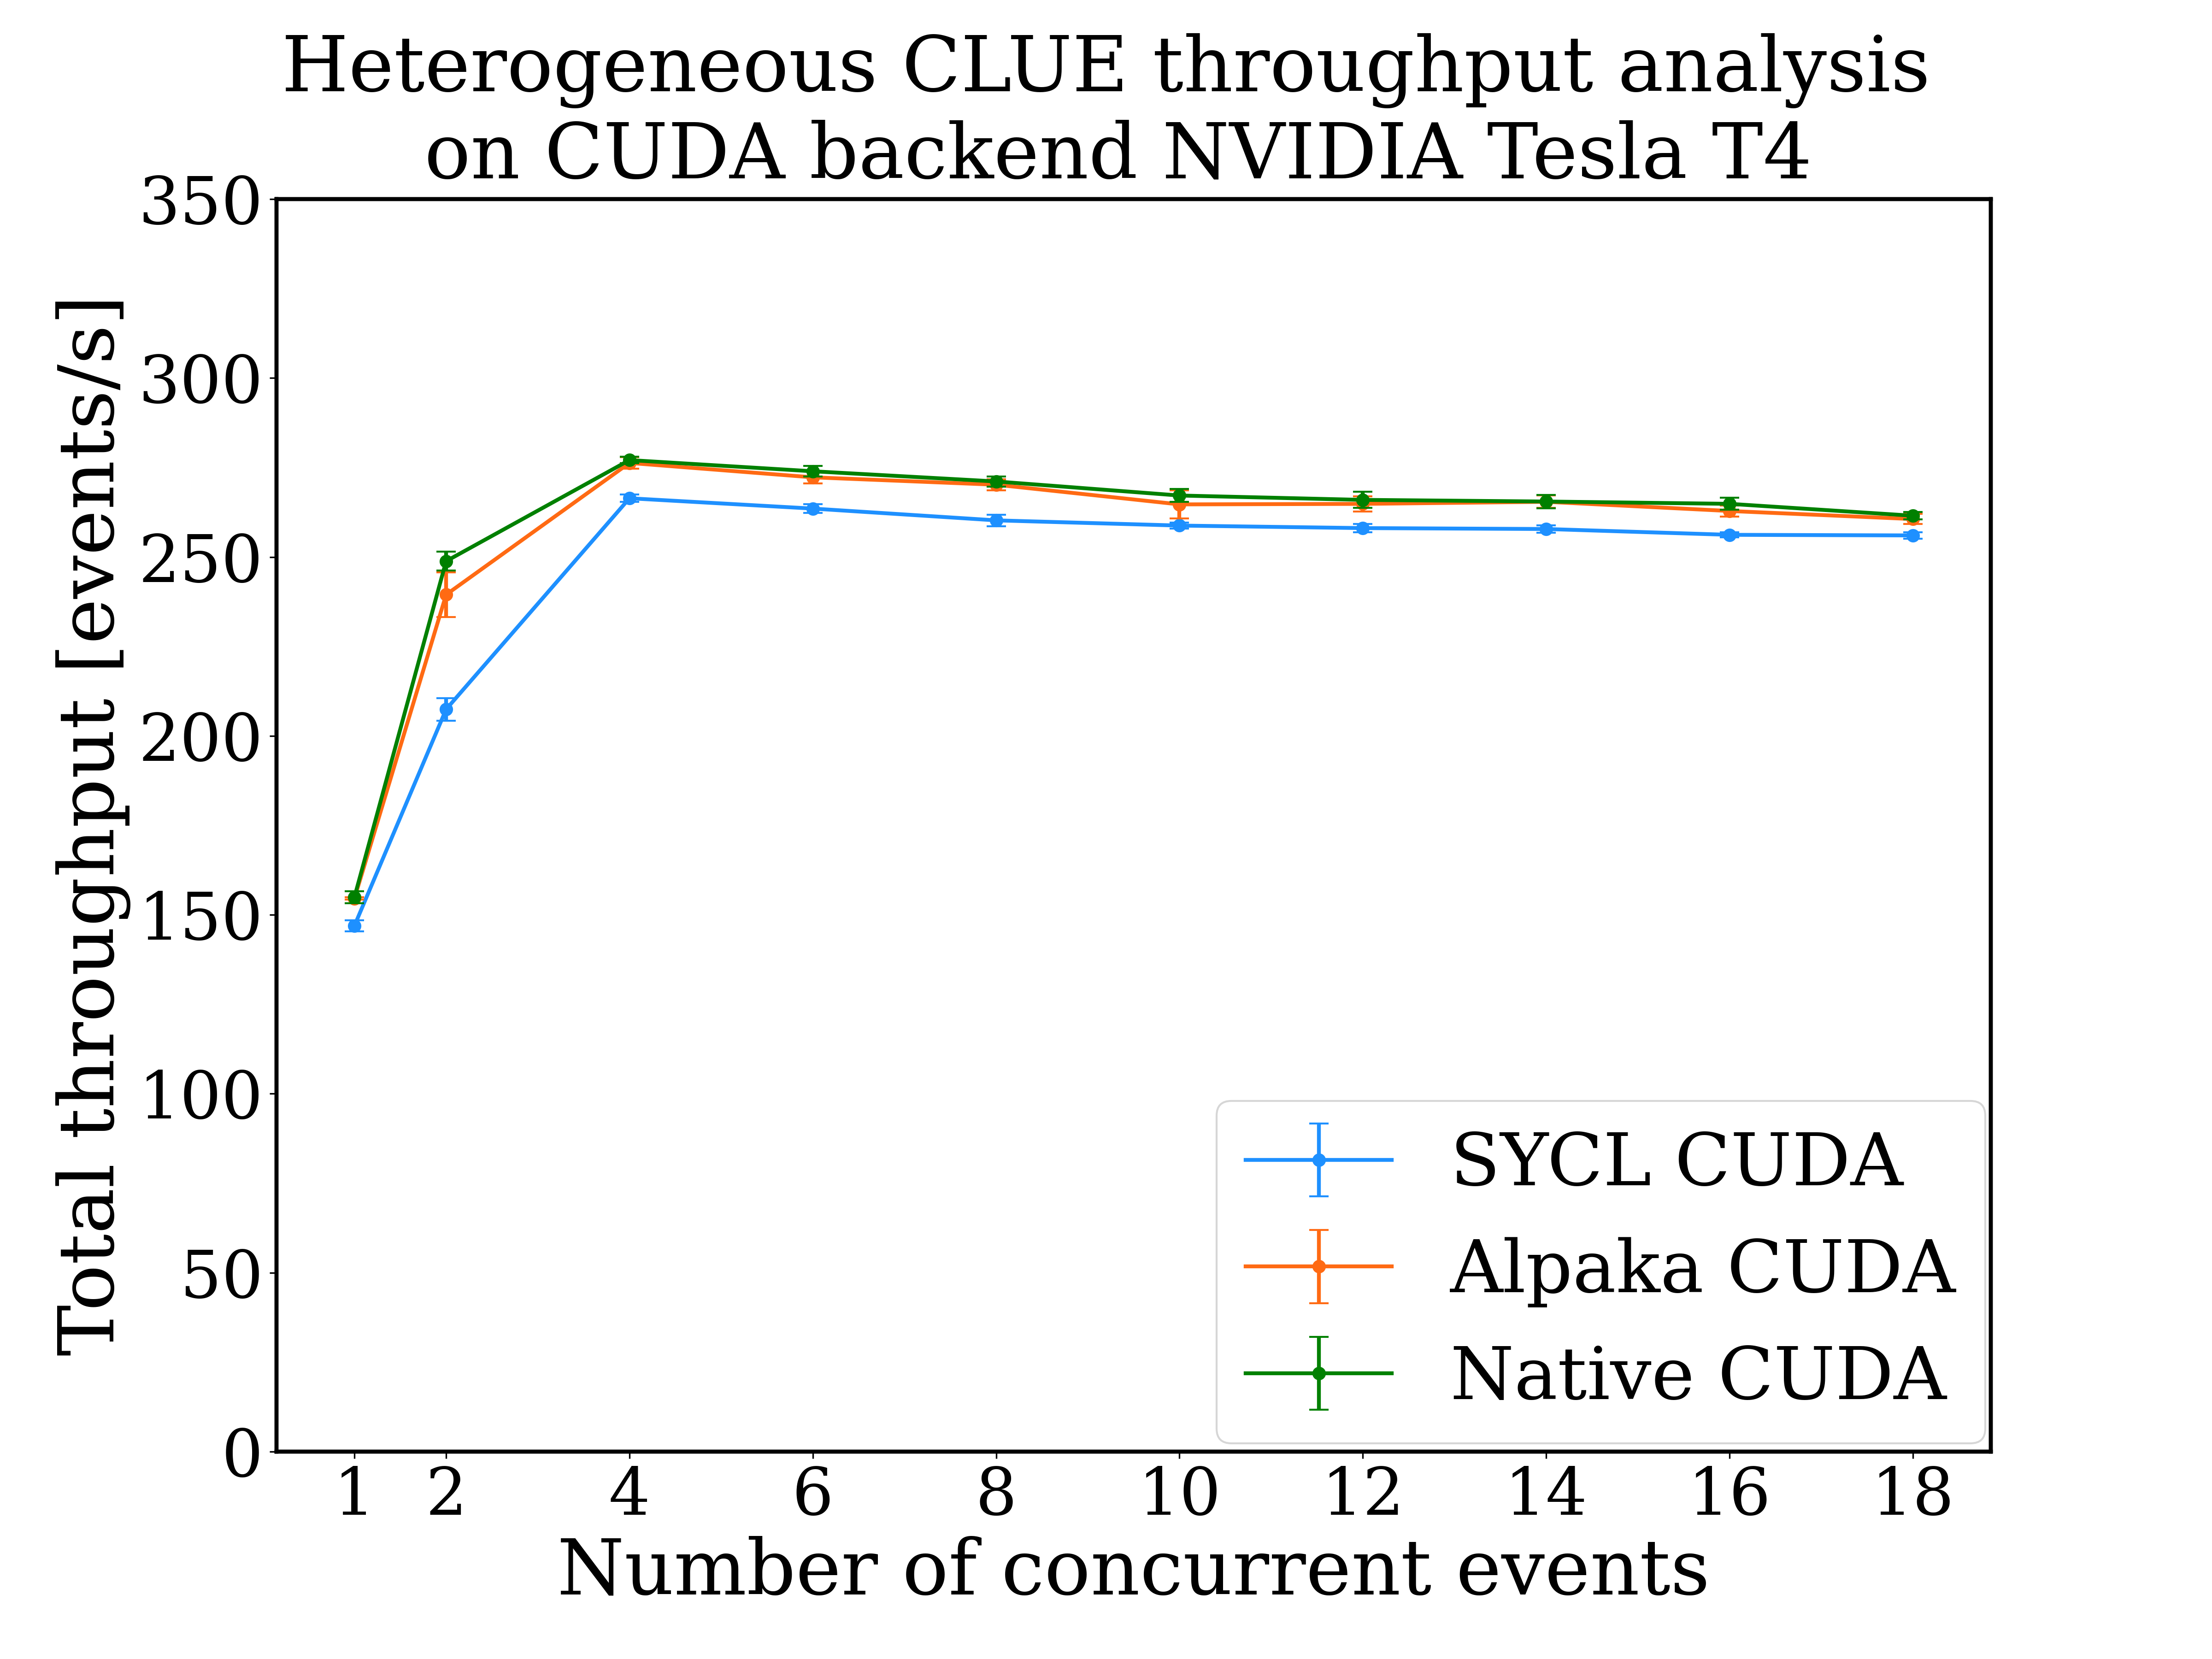
\includegraphics[width=\textwidth]{media/presentazione/hCLUE_cuda_performance.png}
    \caption{Su GPU, SYCL è molto vicino alle performance del codice nativo e di Alpaka.}
    \end{subfigure}
\end{figure}
    
\end{frame}

\begin{frame}{Conclusioni}

\begin{itemize}
    \item I futuri aggiornamenti di LHC comporteranno \textbf{sfide computazionali senza precedenti} per la ricostruzione online e offline
    \item Soluzione: \textbf{calcolo eterogeneo}. Richiede di produrre e mantenere \textbf{codice diverso per ogni dispositivo}
    \item SYCL consente di scrivere un \textbf{unico codice eseguibile da sistemi eterogenei}
    \item Le \textbf{performance} mostrate da CLUE sono \textbf{incoraggianti}
     \item Lo standard è in \textbf{continuo aggiornamento}
    \item \textbf{Progetti più estesi} sono \textbf{in sviluppo} per valutare le potenzialità di SYCL
    
\end{itemize}
    
\end{frame}

\end{document}